\section{Theorie}
\label{sec:theorie}


Schallwellen sind longitudinale Wellen, die in der Form
\begin{equation}
    p(x, t) = p_0 + v_0 Z \cos(\omega t - k x)
    \label{eq:druckwelle}
\end{equation}
als Druckschwankungen im Raum propagieren.

Die akustische Impedanz $Z = c \rho$ beschreibt dabei den
Widerstand, die Schallwellen im Medium der Dichte $\rho$ %Korrektur
erfahren.
Dabei ist die Schallgeschwindigkeit $c$ materialabhängig. In einer
Flüssigkeit bestimmen die Kompressibilität $\kappa$ %Korrektur
und Dichte über
\begin{equation}
    c_\text{Fl} = \sqrt{\frac{1}{\kappa \rho}}
\end{equation}
die Schallgeschwindigkeit. \\

In Festkörpern bestehen Schallwellen dagegen nicht nur aus 
Longitudinal-, sondern auch aus Transversalwellen. %Hier ist für mich nichts falsch 
Hier gilt
\begin{equation}
    c_\text{Fk} = \sqrt{\frac{E}{\rho}} \,,
\end{equation}
wobei das Elastizitätsmodul $E$ anstelle der Kompressibilität
$\kappa$ eine Rolle spielt. \\


\subsection{Reflexion}

Trifft eine Schallwelle auf eine Grenzfläche, wird ein Teil
reflektiert, der andere wird transmittiert und teilweise
absorbiert.
Mit der akustischen Impedanz $Z_i$ des Mediums $i$ ergibt sich
der Reflexionskoeffizient aus
\begin{equation}
    R = \left(\frac{Z_1 - Z_2}{Z_1 + Z_2}\right)^2 \,.
    \label{eq:reflexkoeff}
\end{equation}

\subsection{Transmission und Absorption}

Der Anteil der Welle, der nicht reflektiert, sondern%Hier ist für mich nichts falsch 
transmittiert wird, bestimmt sich dann aus          %Hier ist für mich nichts falsch

\begin{equation}
    T = 1 - R\, .  %Korrektur
    \label{eq:transmisskoeff}
\end{equation}


Über eine Strecke $x$ verliert eine Schallwelle einen Teil ihrer
Energie durch Absorption. Mit einer Anfangsintensität $I_0$ gilt %Korrektur
\begin{equation}
    I(x) = I_0 \mathrm{e}^{-\alpha x} \,.
\end{equation}

Dabei ist $\alpha$ der Absorptionskoeffizient des Mediums.

\subsection{Durchschallungsverfahren}

Bei dem Durchschallungsverfahren befindet sich der Sender gegenüber
vom Empfänger.
Ein ausgesendeter Impuls, der auf ein Hindernis trifft, kommt
also mit geringerer IntensitäI am Detektor an.          %Korrektur
Der Empfangsimpuls ist, wie in \autoref{fig:abb1} zu erkennen,%Korrektur
niedriger als der Sendeimpuls.

\begin{figure}
    \centering
    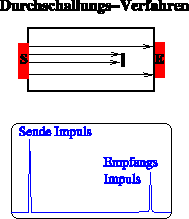
\includegraphics{figures/abb1.pdf}
    \caption{Empfangsbild beim Durchschallungsverfahren \cite{ap06}.}
    \label{fig:abb1}
\end{figure}

\subsection{Impuls-Echo-Verfahren}

Mit einem piezo-elektrischen Kristall als Ultraschallsender und
-empfänger, der in einem elektrischen Feld zu Schwingungen
angeregt werden kann und Ultraschallwellen abstrahlt, wird ein
Ultraschallimpuls ausgesendet. \\

Wie in \autoref{fig:abb2} dargestellt, entsteht bei Reflexion am Hindernis am Detektor ein geringer
Impuls, der Fehlstelle genannt wird, bevor der eigentliche Ausgangsimpuls
wieder am Empfänger ankommt.

\begin{figure}
    \centering
    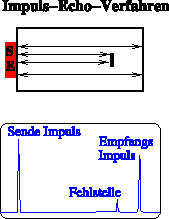
\includegraphics{figures/abb2.pdf}
    \caption{Empfangsbild beim Impuls-Echo-Verfahren \cite{ap06}.}
    \label{fig:abb2}
\end{figure}

So kann z.B. bei bekannter Schallgeschwindigkeit mithilfe von
\begin{equation}
    s = \dfrac{1}{2} c \Delta t
    \label{eq:schallges}
\end{equation}
die Dicke des durchgeschallten Materials bestimmt werden. 

